\documentclass[11pt,a4paper]{article}
\usepackage[T1]{fontenc}
\usepackage[margin=2.3cm]{geometry}
\usepackage{amsmath,amssymb}
\usepackage{graphicx}
\usepackage[dvipsnames]{xcolor}
\usepackage{enumitem}
\usepackage[colorlinks=true,linkcolor=blue,urlcolor=blue]{hyperref}
\setlength{\parskip}{0.6em}
\setlength{\parindent}{0pt}
\begin{document}

\begin{center}{\LARGE\bfseries openeclipse}\\[0.4em]{\large Predict when and where the Moon hides the Sun, in three sessions.}\\[0.2em]\small PAN IIT OSS explainer \textbullet{} secondary school to diploma / undergraduate (levels 3-5)\end{center}

\section*{Why this exists}
An eclipse is a shadow: the Moon's shadow falling on the Earth, or the Earth's shadow falling on the Moon. This explainer shows the geometry behind it, using angles, similar triangles and a few lines of Python, so you can predict eclipses yourself. Never look at the Sun without certified eclipse glasses.

\section*{The end goal}
Predict when and where an eclipse will be seen. The end goal is to predict when and where an eclipse will be seen, and to understand why eclipses repeat every 18 years. The same ideas (orbital periods that almost match) are used in satellite orbits and in spotting patterns in any periodic data.

\section*{How the three sessions build up}
\begin{enumerate}[nosep]
\item \textbf{Session 1: Two discs in the sky, one shadow on the ground} (Level 1, conceptual interactive model, 60 min).
\item \textbf{Session 2: Shadow cones and the eclipse limit} (Level 2, mathematical engineering model, 75 min).
\item \textbf{Session 3: Predicting eclipses and the Saros} (Level 3, simulation and validation, 90 min).
\end{enumerate}

\section{Session 1: Two discs in the sky, one shadow on the ground}

\subsection*{A. Real-world problem}
Once or twice a year, somewhere on Earth, the daytime sky goes dark for a few minutes. The Sun is about 400 times wider than the Moon, so how can the Moon hide it completely? And why does it happen only along a thin track on the ground? SAFETY: looking at the Sun without certified eclipse glasses damages eyes, even when the Sun is mostly covered. Everything in this repo is calculation; you never need to look at the Sun. Health note: this is general education only.

\subsection*{B. Concept and theory}
A solar eclipse happens when the Moon passes between the Sun and the Earth, so the Moon's shadow sweeps across the ground. A lunar eclipse happens when the Moon passes into the Earth's shadow. What decides the sight is the angular size of each disc: a ball of radius r at distance d spans an angle with tan(angle) = r/d. The Sun is 400.7 times wider than the Moon but 389.2 times farther away, so both look about 0.5 degrees wide: 0.533 degrees for the Sun and 0.518 degrees for the Moon at its mean distance. Call the angular radii rs (Sun) and rm (Moon) and the distance between the two disc centres sep. If sep is at least rs + rm there is no eclipse; if the Moon is the bigger disc and sep is at most rm - rs the Sun is totally hidden; if the Moon is the smaller disc and sep is at most rs - rm a bright ring is left (annular); anything between is partial. The Moon is bigger than the Sun only when it is nearer than 373,355 km.

\begin{itemize}[nosep]
\item r: radius of the Sun or Moon (696000 km, 1737 km) (km)
\item d: distance to the Sun or Moon (km)
\item rs, rm: angular radius of the Sun, of the Moon (degrees)
\item sep: angular distance between the two centres (degrees)
\item v: orbital speed of the Moon (1.023 km/s) (km/s)
\end{itemize}

\begin{equation*}
\tan\alpha=\frac{r}{d}
\end{equation*}

\begin{equation*}
\text{total: } r_m\ge r_s \text{ and } \mathrm{sep}\le r_m-r_s;\qquad \text{annular: } r_s>r_m \text{ and } \mathrm{sep}\le r_s-r_m
\end{equation*}

\begin{equation*}
d_{\mathrm{crit}}=\frac{R_{\mathrm{Moon}}}{\tan r_s}
\end{equation*}

\begin{center}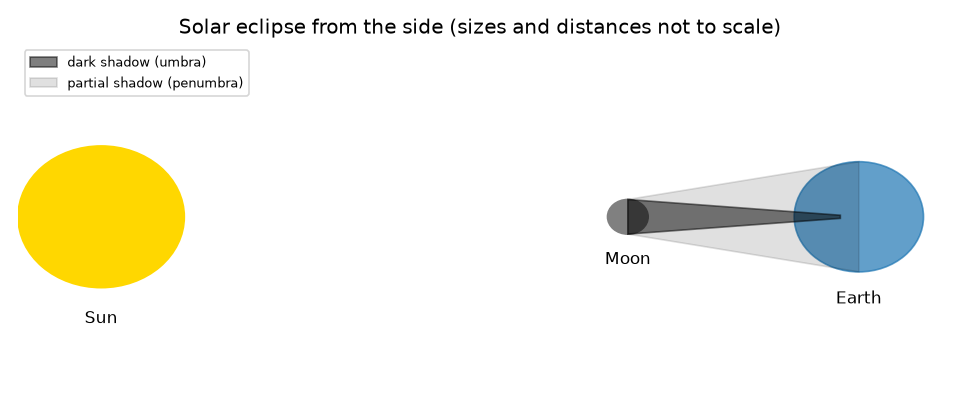
\includegraphics[width=0.85\linewidth]{figures/s01_eclipse_geometry.png}\\\small Solar eclipse from the side (not to scale): dark umbra and partial shadow.\end{center}

\subsection*{E. Worked example}
The Moon is at its mean distance 384400 km and its centre is 0.30 degrees from the centre of the Sun. What kind of eclipse is this and how much of the Sun's area is hidden?
\begin{enumerate}[nosep]
\item Sun: rs = arctan(696000 / 1.496e8) = 0.2666 degrees. Moon: rm = arctan(1737 / 384400) = 0.259 degrees.
\item rs + rm = 0.525 degrees. Since sep = 0.30 is smaller than that, the discs overlap: an eclipse of some kind.
\item rm is smaller than rs and sep is larger than rs - rm = 0.008 degrees, so the Sun is not fully hidden and no ring forms: partial.
\item The overlap of two circles gives a covered fraction of 0.306 of the Sun's area (about 31 percent).
\end{enumerate}
\textbf{Answer.} A partial eclipse with about 31 percent of the Sun's area covered.

\subsection*{F. Questions}
\begin{enumerate}[nosep]
\item \textbf{Conceptual.} The Sun is about 400 times wider than the Moon. Why can the Moon still hide it?
\item \textbf{Numerical.} The Moon is at 400000 km with its centre exactly on the Sun's centre. Find rm and the fraction of the Sun's area covered.
\item \textbf{Graph and simulation interpretation.} On the graph of covered fraction against centre distance for the mean Moon, at about what distance does the curve reach zero? Why is the curve 'flat' at the left end for a Moon at 360000 km?
\item \textbf{Design and optimisation challenge.} Design: a photographer wants a total eclipse from a spot where the discs line up exactly. What condition must the Moon's distance satisfy, and how well must the discs be aligned if the Moon is at 360000 km?
\end{enumerate}

\section{Session 2: Shadow cones and the eclipse limit}

\subsection*{A. Real-world problem}
Why is a total solar eclipse so rare at any one place, and why is there not an eclipse every month? The Moon's dark shadow is a thin cone whose tip only just reaches the Earth, and the Moon's orbit is tilted, so most new moons pass above or below the Sun. SAFETY: never look at the Sun without certified eclipse glasses. This is general education and simplified geometry, not a tool for planning where to stand.

\subsection*{B. Concept and theory}
Let R and r be the Sun's and Moon's radii and D the Sun-Moon distance. Draw the line from the top of the Sun to the top of the Moon and continue it to the axis: the tip of the dark cone, at distance L behind the Moon. The small triangle (tip to Moon) and the big triangle (tip to Sun) are similar, so r/L = R/(L + D), which gives L = D r / (R - r) = 374,289 km. That is 10,111 km short of the mean Earth-Moon distance 384,400 km: at the mean distance the tip falls short of the ground (which starts 378,022 km from the Moon) and the eclipse is annular. The dark circle on the ground has radius r (L - s)/L at distance s behind the Moon; negative means beyond the tip (the ring region, the antumbra). It is positive only if the Earth-Moon distance is below L + 6378 = 380,667 km. At perigee, 356500 km, the dark path is 224 km wide. The penumbra radius at the ground is 3500 km. The Moon's orbit is tilted by i = 5.145 degrees to the ecliptic, so its ecliptic latitude at angle u from the node is sin(beta) = sin(i) sin(u). A partial eclipse needs \textbar{}beta\textbar{} below pi + rs + rm, where pi (0.951 degrees at the mean distance) is the parallax of the Moon; the limit is 1.476 degrees, giving u up to 16.7 degrees. A central eclipse needs \textbar{}beta\textbar{} below pi, giving 10.7 degrees. With the extremes of distance and tilt the partial limit reaches 18.4 degrees, is certain within 15.4 degrees, and the central limit reaches 11.8 degrees. The Sun passes a node twice per draconic year of 346.62 days, so eclipse seasons are 173.31 days apart.

\begin{itemize}[nosep]
\item R, r: radius of the Sun, of the Moon (696000, 1737) (km)
\item D: Sun-Moon distance (1.496e8) (km)
\item L: length of the umbra behind the Moon (km)
\item s: distance behind the Moon (km)
\item d: Earth-Moon distance (km)
\item i: tilt of the Moon's orbit (5.145) (degrees)
\item u: angle from the node along the orbit (degrees)
\item beta: ecliptic latitude of the Moon (degrees)
\item pi: parallax of the Moon, arcsin(6378 / d) (degrees)
\end{itemize}

\begin{equation*}
L=\frac{D\,r}{R-r}
\end{equation*}

\begin{equation*}
\rho_{\mathrm{umbra}}(s)=r\,\frac{L-s}{L},\qquad \rho_{\mathrm{penumbra}}(s)=r+s\,\frac{R+r}{D}
\end{equation*}

\begin{equation*}
|\beta|<\pi+s_{\odot}+s_{\mathrm{M}},\qquad \sin\beta=\sin i\,\sin u
\end{equation*}

\begin{equation*}
u_{\mathrm{limit}}=\arcsin\!\left(\frac{\sin\beta_{\mathrm{limit}}}{\sin i}\right)
\end{equation*}

\begin{equation*}
T_{\mathrm{season}}=\frac{2u_{\mathrm{limit}}}{360^\circ/346.62\ \mathrm{d}}
\end{equation*}

\begin{center}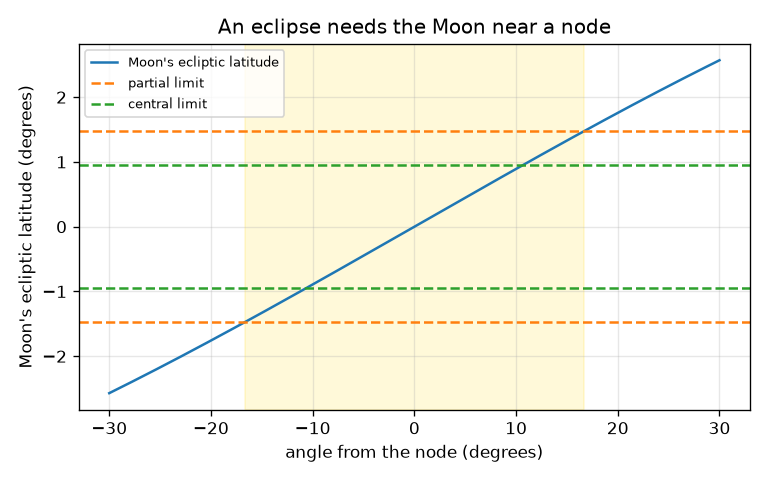
\includegraphics[width=0.85\linewidth]{figures/s02_eclipse_limit.png}\\\small The Moon's ecliptic latitude against the angle from the node, with the partial and central limits.\end{center}

\subsection*{E. Worked example}
The Moon is at perigee, 356500 km from the Earth. How wide is the path of totality, and how long does totality last at the equator?
\begin{enumerate}[nosep]
\item Umbra length: L = 1.496e8 * 1737 / (696000 - 1737) = 374,289 km.
\item The nearest ground is s = 356500 - 6378 = 350,122 km behind the Moon, which is less than L, so the eclipse is total.
\item Dark radius: 1737 * (374289 - 350122) / 374289 = 112.2 km, so the path is 224.3 km wide.
\item Shadow speed over the equator ground = 2 pi d / T minus 0.465 km/s = 0.949 - 0.465 = 0.484 km/s.
\item Duration = 224.3 km / 0.484 km/s = 463 s = 7.7 minutes.
\end{enumerate}
\textbf{Answer.} The path is about 224 km wide and totality lasts about 7.7 minutes at most.

\subsection*{F. Questions}
\begin{enumerate}[nosep]
\item \textbf{Conceptual.} At the mean Moon distance the discs look almost equal. Why is an eclipse at the mean distance annular, not total?
\item \textbf{Numerical.} Compute the umbra length for R = 696000 km, r = 1737 km, D = 1.496e8 km and compare it with 384400 km.
\item \textbf{Graph and simulation interpretation.} On the graph of dark-shadow radius against Earth-Moon distance, where does the curve cross zero, and what does a negative value mean?
\item \textbf{Design and optimisation challenge.} Design: how large a limit angle must we assume so that every eclipse season is certain to contain at least one new moon within the limit? Compare 15.4 degrees with the synodic month.
\end{enumerate}

\section{Session 3: Predicting eclipses and the Saros}

\subsection*{A. Real-world problem}
Ancient astronomers predicted eclipses without computers: after about 18 years the Sun, Moon and node return to nearly the same arrangement, so eclipses repeat. Can we rediscover that cycle with a few lines of Python, and predict which new moons in the next years give an eclipse? EDUCATIONAL APPROXIMATION: our model is accurate to hours in time and sometimes wrong about the type; for real dates, times and maps use published eclipse tables. SAFETY: never look at the Sun without certified eclipse glasses.

\subsection*{B. Concept and theory}
Three angles run like clocks from one reference new moon (6 January 2000): the Sun's anomaly M, the Moon's anomaly M' and the Moon's argument of latitude F (angle from the ascending node). Each advances by 360 times the synodic month divided by the period of the clock. The mean new moon time is JD0 + k * 29.530589 days, and seven correction terms (up to 0.4 days) fix the largest wobbles. The Moon's latitude beta comes from F and M' with a short series, its distance from M', and gamma = d sin\textbar{}beta\textbar{} / R\_Earth is the distance of the shadow axis from the Earth's centre in Earth radii. A partial eclipse needs gamma below 1 plus the penumbra radius in Earth radii; a central one needs gamma below 1. Using only the mean motions, the predicted times are wrong by up to 12.7 hours; with the corrections, every one of 13 published eclipses is within 0.2 hours. 223 synodic months are 6585.32 days; 242 draconic months are 6585.36 days and 239 anomalistic months are 6585.54 days: nearly equal. So after 223 new moons (the Saros, 18 years 11 days 7.7 hours when 4 leap days fall in the 18 years) the Moon is again near the same node and the same distance. The extra 0.32 day turns the Earth by 115.7 degrees, so the track moves about 120 degrees west. One Saros moves the Moon 0.478 degrees along its orbit relative to the node, so a series lasts about 69 repeats.

\begin{itemize}[nosep]
\item k: number of the new moon after 6 January 2000 (no unit)
\item M, M', F: Sun anomaly, Moon anomaly, Moon argument of latitude (degrees)
\item beta: ecliptic latitude of the Moon at new moon (degrees)
\item gamma: distance of the shadow axis from the Earth's centre (Earth radii)
\item T\_syn, T\_dra, T\_ano: synodic, draconic, anomalistic month (29.530589, 27.212221, 27.554550) (days)
\item magnitude: fraction of the Sun's diameter covered at the best place (no unit)
\end{itemize}

\begin{equation*}
F_k=F_0+k\,360^\circ\,\frac{T_{\mathrm{syn}}}{T_{\mathrm{dra}}}\ (\mathrm{mod}\ 360^\circ)
\end{equation*}

\begin{equation*}
\gamma=\frac{d\,\sin|\beta|}{R_{\oplus}}
\end{equation*}

\begin{equation*}
223\,T_{\mathrm{syn}}\approx 242\,T_{\mathrm{dra}}\approx 239\,T_{\mathrm{ano}}
\end{equation*}

\begin{equation*}
\Delta\lambda_{\mathrm{track}}=360^\circ\times\left(223\,T_{\mathrm{syn}}\ \mathrm{mod}\ 1\ \mathrm{day}\right)
\end{equation*}

\begin{center}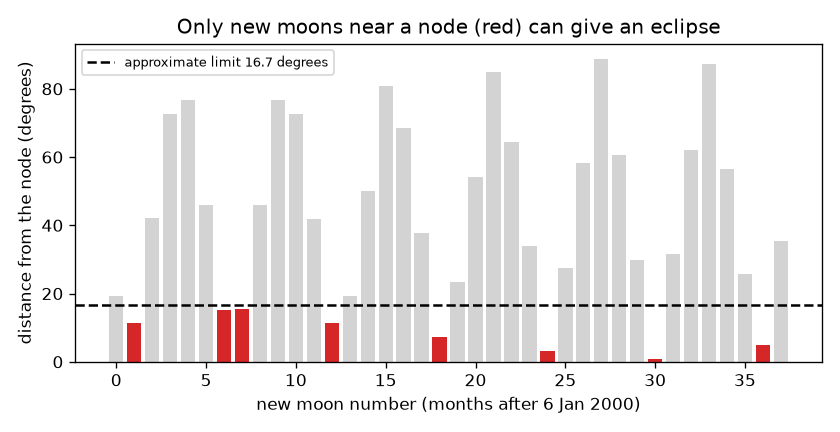
\includegraphics[width=0.85\linewidth]{figures/s03_node_distance.png}\\\small Distance from the node for 38 new moons: red bars can give an eclipse.\end{center}

\subsection*{E. Worked example}
Predict the new moon of the total eclipse of 8 April 2024 and compare it with the published greatest-eclipse time of 18:17 UT.
\begin{enumerate}[nosep]
\item The nearest new moon number is k = 300. Mean time: 2451550.09766 + 300 * 29.530589 days = 8 April 2024 18:35 UT.
\item The seven correction terms add -12.4 minutes, giving 18:22 UT. The published time is 18:17 UT: the prediction is within 6 minutes.
\item The argument of latitude at that moment gives a distance from the node of 1.9 degrees, far inside the limit of 16.7 degrees.
\item The latitude series gives beta = 0.36 degrees and the Moon distance 359,808 km, so gamma = 0.35 (below 1: central).
\item The umbra is longer than the Moon distance, so the predicted type is total.
\end{enumerate}
\textbf{Answer.} A total eclipse at about 18:22 UT, 6 minutes from the published time, with gamma 0.35.

\subsection*{F. Questions}
\begin{enumerate}[nosep]
\item \textbf{Conceptual.} Why does using only the mean motion give an error of up to 12.7 hours in the time of new moon?
\item \textbf{Numerical.} Compute 223 synodic months and 242 draconic months in days with the stated mean periods. How far apart are they?
\item \textbf{Graph and simulation interpretation.} In the Saros-series figure, how many degrees does the Moon move past the node per member, and about how many members does a series have inside the 16.7 degree limit?
\item \textbf{Design and optimisation challenge.} Design: you want to find an eclipse whose track returns to nearly the same longitude as an earlier one. Which multiple of the Saros should you use, how many years is it, and how close is the longitude?
\end{enumerate}

\section{Real-world mini-project}
\textbf{Which new moons in 2027 to 2029 can give a solar eclipse?.} Use the Session 3 functions to list every new moon from 1 January 2027 to 31 December 2029 that falls in an eclipse season, with the predicted type (partial, annular, total) and gamma. This is an educational approximation, accurate to hours in time and sometimes wrong about the type: label your table that way, and tell the reader to check published eclipse tables (for example the NASA eclipse website) for real dates, times and maps. Safety: never look at the Sun without certified eclipse glasses.

\section{The path ahead}
\begin{enumerate}[nosep]
\item \textbf{Session 4: Minute-level timing.} A longer series for the new moon time and the Moon's latitude, checked against published eclipses.
\item \textbf{Session 5: Every type right.} An improved classifier for total, hybrid, annular and partial eclipses.
\item \textbf{Session 6: The footprint on a rotating Earth.} A simulation of the umbra footprint for one eclipse, drawn on a world outline.
\item \textbf{Session 7: Build a whole Saros series.} A listing of every member of one series with its type, gamma and magnitude.
\item \textbf{Session 8: Lunar eclipses as the other half.} A predictor for lunar eclipses in the same 3-year window.
\end{enumerate}

\section{Answers and hints}

\subsection*{Session 1}
\begin{enumerate}[nosep]
\item \textbf{Conceptual.} Hint: Compare the ratio of the diameters with the ratio of the distances. Solution: The apparent size depends on size divided by distance. The diameter ratio is 400.7 and the distance ratio is 389.2, almost the same, so the two discs look about equally wide: 0.533 degrees and 0.518 degrees. Because the Moon's distance varies, it is sometimes slightly bigger than the Sun (total eclipse) and sometimes slightly smaller (annular).
\item \textbf{Numerical.} Hint: rm = arctan(1737 / d); if the smaller disc sits fully inside the larger one, the fraction is (small radius / large radius) squared. Solution: rm = arctan(1737 / 400000) = 0.2488 degrees. Since rm is smaller than rs = 0.2666 the Moon sits inside the Sun's disc: annular. Covered fraction = (0.2488 / 0.2666)\textasciicircum{}2 = 0.871, so 87.1 percent. Sanity check: it is below 100 percent, as a ring of Sun remains.
\item \textbf{Graph and simulation interpretation.} Hint: Use the sum of angular radii; for the second part compare rm - rs with the flat stretch. Solution: It reaches zero at sep = rs + rm = 0.525 degrees, when the edges just touch. For a Moon at 360000 km the Moon is bigger than the Sun by 0.0099 degrees, so for any sep from 0 up to 0.0099 degrees the whole Sun is hidden and the curve stays at 1 (100 percent).
\item \textbf{Design and optimisation challenge.} Hint: Total needs rm at least rs; then sep must not exceed rm - rs. Solution: The Moon must be nearer than 373,355 km, so that rm is at least rs. At 360000 km, rm - rs = 0.0099 degrees, so the centres must be within 0.0099 degrees of each other. Trade-off: a closer Moon gives a larger margin, so the total phase is longer and the track wider (Session 2).
\end{enumerate}

\subsection*{Session 2}
\begin{enumerate}[nosep]
\item \textbf{Conceptual.} Hint: Compare the umbra length with the distance from the Moon to the nearest ground. Solution: The umbra is L = 374,289 km long, but the nearest ground is 378,022 km behind the Moon, so the tip stops 3,733 km short of the ground and the observer is inside the antumbra, seeing a ring. A total eclipse needs the Moon nearer than 380,667 km, which happens near perigee.
\item \textbf{Numerical.} Hint: L = D r / (R - r). Solution: L = 1.496e8 * 1737 / 694263 = 374,289 km, about 3.7e5 km. It is 10,111 km shorter than 384400 km. Units: kilometres, same as the inputs.
\item \textbf{Graph and simulation interpretation.} Hint: The crossing is where the tip just touches the ground. Solution: It crosses zero at 380,667 km (L + 6378 km). Below that the radius is positive: total eclipse. Above it the value is negative: the ground is beyond the tip, inside the antumbra, and the eclipse is annular; the magnitude is the radius of the ring region (17.3 km radius at the mean distance, so 34.6 km wide).
\item \textbf{Design and optimisation challenge.} Hint: Season length = 2 limit / (360 / 346.62) days; compare with 29.53 days. Solution: With the certain limit 15.4 degrees the season lasts 29.65 days, a little longer than the 29.53 day synodic month, so at least one new moon falls in every season. With the mean limit 16.7 degrees the season is 32.1 days, so sometimes two new moons fit. Trade-off: a larger limit gives a longer season but also includes eclipses that are tiny partials.
\end{enumerate}

\subsection*{Session 3}
\begin{enumerate}[nosep]
\item \textbf{Conceptual.} Hint: Think about what a 'mean' motion leaves out: the Moon and the Earth do not move at constant speed. Solution: The Moon speeds up near perigee and slows near apogee, and the Earth speeds up near perihelion, so the real new moon is ahead of or behind the evenly spaced mean new moon by up to about half a day. The seven correction terms (dominated by -0.4072 sin M') capture most of this, bringing the error down to 0.2 hours for our 13 test eclipses.
\item \textbf{Numerical.} Hint: Multiply and subtract. Solution: 223 * 29.530589 = 6585.32 days and 242 * 27.212221 = 6585.36 days. They differ by 0.036 days (about 52 minutes). The anomalistic count 239 * 27.554550 = 6585.54 days is 0.216 days (5 hours) away. All three agree to within a fraction of a day.
\item \textbf{Graph and simulation interpretation.} Hint: Count how many steps of the drift fit into the width of the window, 2 * 16.7 degrees. Solution: The drift is 0.478 degrees per Saros (from 360 * (223 T\_syn / T\_dra - 242)). The window is 33.4 degrees wide, and 33.4 / 0.478 = 69 members. Real series differ, because the limit depends on the Moon and Sun distance.
\item \textbf{Design and optimisation challenge.} Hint: One Saros shifts the track by 115.7 degrees west; find a multiple close to 360 degrees. Solution: Three Saros periods shift the track by 347.1 degrees, which is 12.9 degrees short of a full circle, so the track returns to within 13 degrees of the start. Three Saros periods are 19755.96 days, that is 54.09 years. Trade-off: longer spans repeat the same longitude but the series drifts out after about 69 repeats, so it is only usable within a series.
\end{enumerate}

\section{How to join}
Read \texttt{CONTRIBUTING.md} in the repository, then pick an issue labelled \texttt{good first issue}. Repository: \url{https://github.com/KrunalPanchal1995/openeclipse}

\end{document}
